%# -*- coding: utf-8-unix -*-
% !TEX program = xelatex
% !TEX root = ../thesis.tex
% !TEX encoding = UTF-8 Unicode

\section{概述}%intro
\label{sec:tabel-intro}

% basic introduction to table linking

海量的互联网文本信息中,充斥着以HTML编写的表格,
即互联网表格\cite{cafarella2008webtables,wang2012understanding}。
和纯文本相比,互联网表格中的行列形式携带了非常有价值的结构化信息。
为了能让机器理解,并且很好的处理表格中的信息,%~\parencite{wang2012understanding},
第一个步骤就是需要识别每个单元格中文本内容所对应的实体,
并映射到一个标准词库,或是知识库上,例如维基百科或Freebase。
这样的一个在互联网表格上进行实体链接的任务,
在本章节被称为表格链接\cite{bhagavatula2015tabel,wu2016entity}。

对于表格链接任务,
已有的研究工作\cite{bhagavatula2015tabel,limaye2010annotating}主要针对英文表格,
由于使用知识库也为英文,表格链接是在单一语言场景中进行的。
然而,当需要链接的表格以其它语言编写的时候,
对应语言的非英文知识库往往不够全面,无法涵盖目标表格中提及的所有实体。
例如中文版维基百科,其中包含的实体(页面)数量仅为英文维基百科的1/6左右。
%多聊几句?
基于不同语言知识库大小上的差异,
本章探寻一种全新的方式将非英文表格与英文知识库相连,
该任务也被称为\textbf{跨语言表格链接}。
如\figref{fig:tabel-intro}所示,
中文表格里的电影 ``{邮差}'' 在中文维基百科里没有对应的实体,
但存在对应的英文维基实体 ``Il Postino: The Postman'' ,
因此可以建立跨语言的链接。

\begin{figure}[th]
\centering
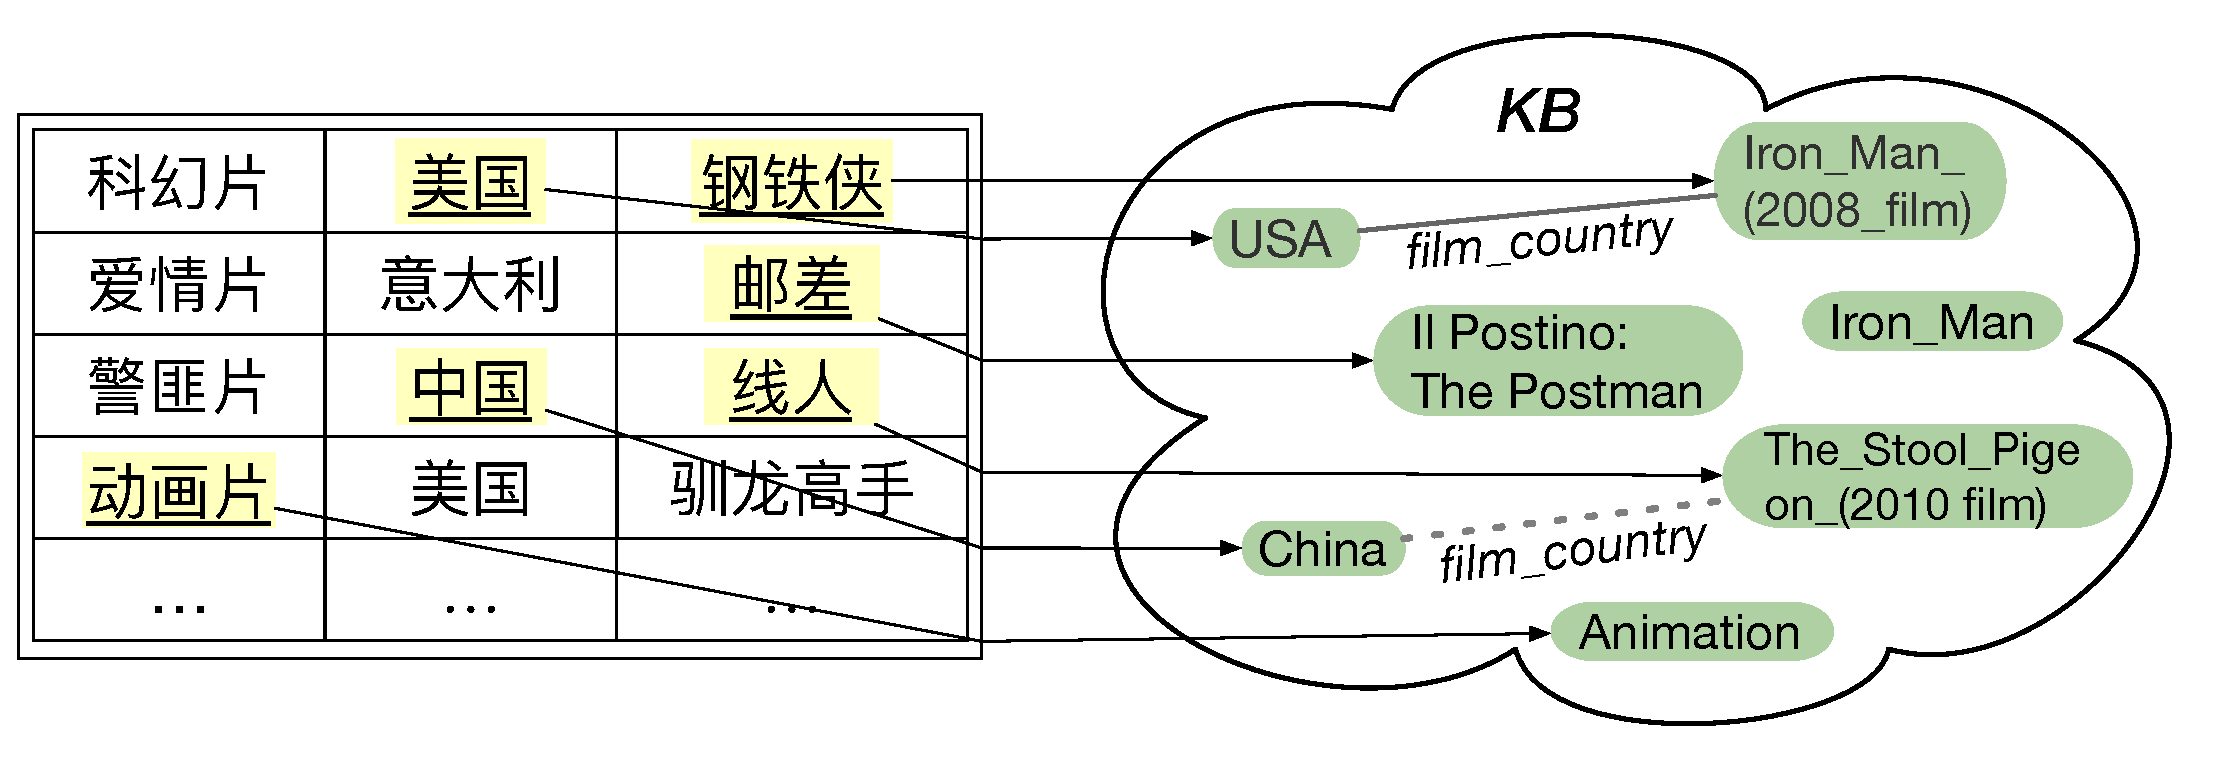
\includegraphics[width=0.9\columnwidth]{figure/tabel/intro.eps}
%\scalebox{0.22}{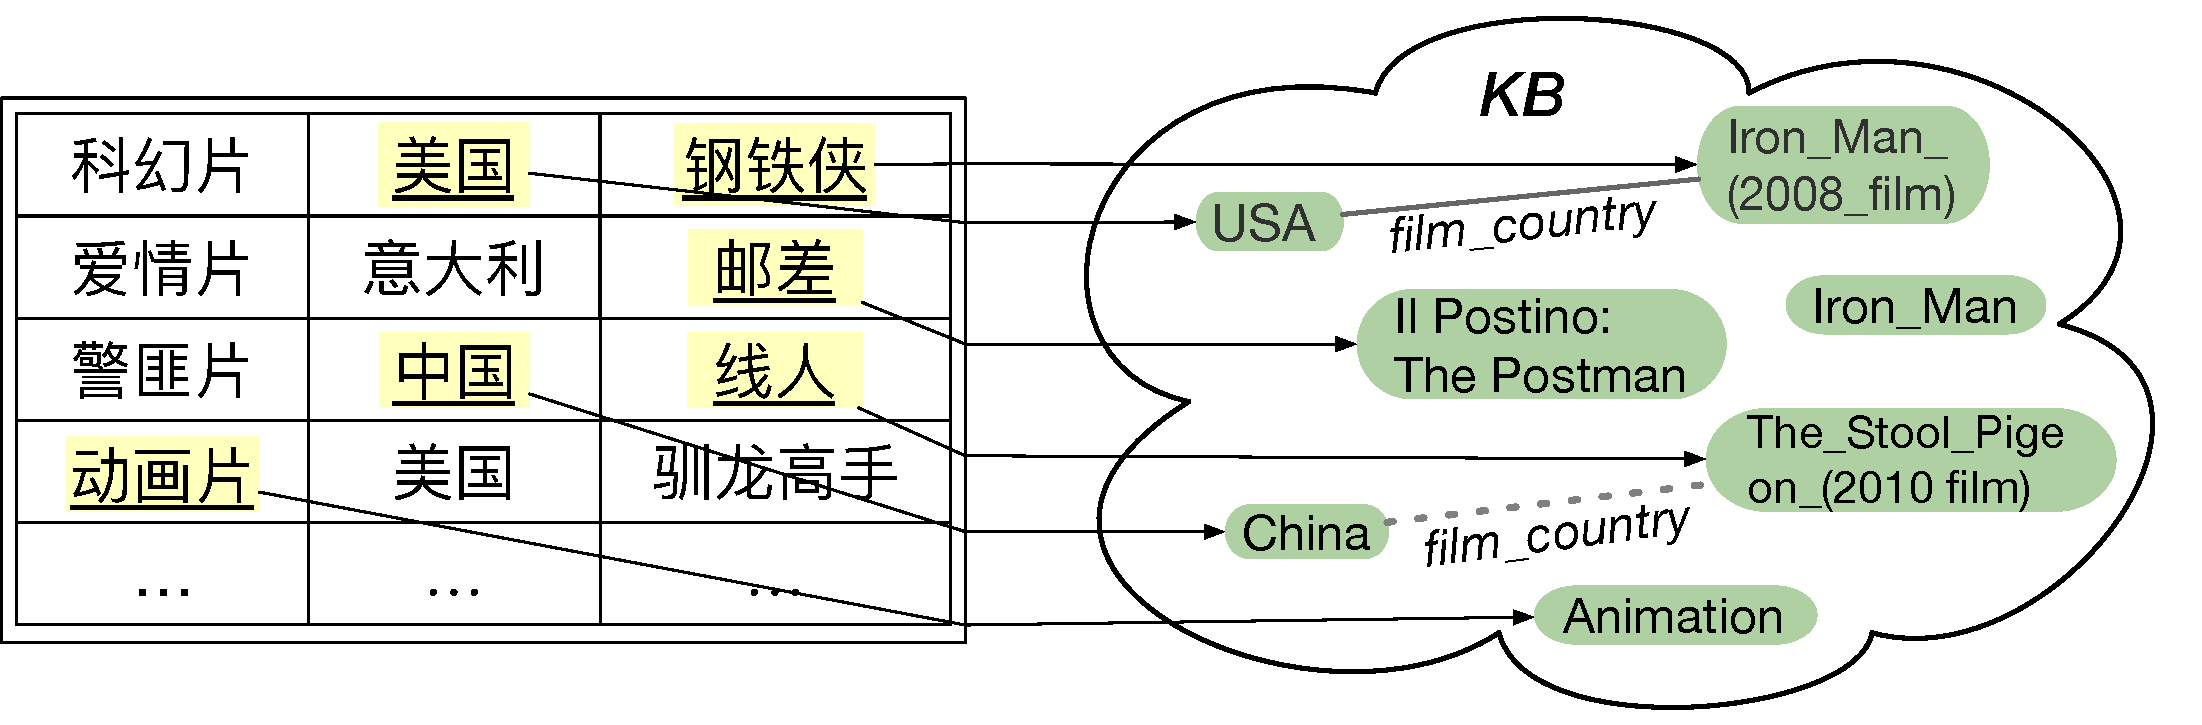
\includegraphics[angle=0]{figure/tabel/intro.pdf}}
\bicaption{中文表格到英文知识库的跨语言链接示例。}
{Example of cross-lingual table linking from Chinese to English.}
\label{fig:tabel-intro}
\end{figure}

帮助目标知识库补充事实三元组,是我们尝试跨语言表格链接的另一个动机。
英文知识库比其它语言知识库更加庞大,也更加结构化,但仍然包含许多长尾实体。
这些实体仅出现知识库的极少数事实三元组中,例如别国的电影、名人等,
考虑到英文知识库的贡献者更多以英语为母语,这些实体的相关信息就很容易被忽略。
另一方面,海量非英文的互联网表格成为了与长尾实体相关的丰富的语义信息来源。
例如,\figref{fig:tabel-intro}描述了电影与它的原产国之间的关系。
国产电影 ``{线人}'' 有对应的英文维基页面 ``The\_Stool\_Piegon\_(2010\_film)'' ,
但与之相应的Freebase实体却缺少许多相关的知识。
若我们准确将该电影链接至维基百科,
并根据表格前两列的多个实体对推理出关系$film\_country$,
那么就可为知识库补充新的事实。

%In this paper, we attempt to solve the cross-lingual table linking problem
%{\em without} using any non-English knowledge bases.
%%That is, our goal is to link the mentions in the non-English table 
%%directly to an entity in the English knowledge base. 
%%The advantage of this is we do not discard any information of non-English mentions
%%so that our model has the ability to tolerate the error caused by translation.
%To the best of our knowledge, this is the first attempt that attacks the 
%cross-lingual table linking problem. 


具体论述我们提出的跨语言表格链接方法之前,首先来讨论两种朴素的做法。
第一种方式主要基于已有单一语言的表格链接技术,
将表格映射到语言一致的非英文知识库,
然后再利用知识库之间存在的跨语言链接,%~\parencite{tsai2016cross},
将实体翻译至英文知识库。
例如不同语言的维基百科之间就存在着人工编辑好的跨语言链接。
这种方式的主要问题在于:
1) 非英文知识库的信息量较低,可能无法覆盖每一个单元格的实体;
2) 并不是每个非英文知识库都会存在和跨语言链接。

第二种做法中,整个非英文表格的内容首先直接被翻译成英文,
然后整个问题便退化成英文上的表格链接,以往方法可以直接套用。%\parencite{mcnamee2011cross}。
%这种两阶段方式依然不够有效,
它与远距离监督模型很相似,各单元格的(非英文名称,英文实体)对并不直接作为训练数据。
%翻译过程的错误会被传播到之后的链接步骤,而无法得到反馈。
此法的缺陷在于对已有翻译工具准确率的高度依赖:
一方面,文本翻译过程仅生成单一结果,一旦错误则对后续链接步骤影响很大;
另一方面,翻译工具如同黑盒,无法根据训练数据进行优化。

在本章中,为了使研究具有普适性,我们忽略不同语言知识库之间的跨语言链接,
尝试在\textbf{不使用}任何非英文知识库进行过渡的情况下,解决跨语言的表格链接任务。
据我们所知,本章节提出的解决方案,是对跨语言表格链接的第一次尝试。

对于实体链接任务而言,
%\parencite{tsai2016cross,mcnamee2011cross,bhagavatula2015tabel,wu2016entity},
无论是否跨语言,第一个步骤总是为每个单元格生成一组候选实体,
之后整个任务转换为排序问题,对每单元格寻找与其描述最接近的候选实体。
主要的技术挑战在于表格描述和知识库来自不同的语言,
无法依靠任何字面上的相似特征。
此外,表格中缺少纯文本里的谓语、状语等相关上下文,
给单个实体的消歧义带来了困难。
%The major technical challenge of our task is since the source mention
%and the target entity come from two different languages,
%their feature representations are naturally incompatible. 
%To make matters worse, tables offer very limited context for disambiguating
%a mention in the first place.

%Since the language of source mention and target entity is inconsistent, 
%it's hard to direct use the surrounding infomation of them \XS{rephrase}. 
%Besides, this task still has to face a lack of surrounding contexts 
%which can be very helpful during entity disambiguation in normal entity linking tasks.

% image CNN, table is like image

为了解决上述的两个挑战,
我们提出了基于神经网络的联合模型来解决跨语言表格链接问题,
它具有以下三个特点。
首先,模型主体基于跨语言词向量,我们将单元格的描述短语、%mention
上下文、以及知识库的实体映射到不同语言对应的连续向量空间作为语义特征表示,
并且使用线性变换的方式,实现不同语言的向量空间统一。
其次,模型充分利用表格中同一行列的实体所具有的相关性,
并通过神经网络学习不同粒度的相关性特征。
最后,模型基于联合训练思路,以优化整张表格的匹配程度作为目标函数,
使用成对排序损失函数进行参数学习以及多轮迭代的预测方式,对新的表格完成链接。

%Most existing work \XS{cite} mines hand-crafted features to measure the similarity 
%between mentions and candidate entities.  Since feature engineering suffers XXX, 
%some work attempt to use nerual network \XS{cite} to generate fearures, 
%which shows great improvements in task of entity linking. 
%
%As we should notice, a table can be regarded as a matrix of texts, similar to an image, which is a matrix of pixels. 
%Inspired by that idea of using deep neural networks to capture rich semantics of images, which has been proven successful, 
%we present a jointly modeling framework based on nerual networks to solve our problem.
%Besides, Convolotional Neural Networks(CNN) is a natural structure to deal with data in matrix form such as tables.

% Contribution
本章的贡献可以总结为以下四个部分:
\begin{enumerate}
\item{我们首次尝试在跨语言场景上进行表格链接;}
\item{我们提出了一个基于神经网络的联合训练模型,能有效捕捉原始表格与候选链接表格的语义相关性,
并消除不同语言之间的语义间隔;}%这一段写的很烂,可能要改
\item{联合模型除了捕捉单个单元格描述与候选实体间的语义关联特征,
还提出了一种一致性特征,用于捕捉候选链接表格内部不同实体间的联系,有效提升模型的预测准确率;}
\item{我们构建了从中文到英文的跨语言表格链接数据集用于实验,
本章提出的模型效果显著优于其它基线模型,
同时我们进行了一系列分析实验,以验证模型各部分的有效性。}
\end{enumerate}

%\begin{itemize}
%\item We are the first to define the problem of cross-lingual entity linking 
%for web tables (\secref{sec:problem});
%\item We present a novel neural network based joint model which effectively captures the rich semantics of mention table and referent entity table simultaneously. Based on that, we bridge the gap between different languages in this task (\secref{sec:translation} and \secref{sec:cell});
%\item We propose a coherence feature in the joint linking model which captures the correlation of entities appearing in the same table and improves the linking accuracy (\secref{sec:coherence});
%\item The framework significantly outperforms
%several baseline methods, with an accuracy of 62.9\%. (\secref{sec:eval}).
%%and question answering. Furthermore, our schema representation is
%%on par with the popular word embedding model in computing relation similarity (\secref{sec:eval}).
%\end{itemize}
